\documentclass{article}


%%%%%%%%%%%%%%%%%%%%%%%%%%%%%%%%%%%%%%%%%%%%%%%%%%%%%%%%%%%%
%
% PROSZE NIE WPROWADZAC TUTAJ ZMIAN! ZABAWY TYLKO NA WLASNEJ KOPII
%
%%%%%%%%%%%%%%%%%%%%%%%%%%%%%%%%%%%%%%%%%%%%%%%%%%%%%%%%%%%%

%przykladowe pakiety
\usepackage[utf8]{inputenc}
\usepackage{polski}
\usepackage{graphicx}
\usepackage{amsmath} % w zasadzie tez mozna wywalic 
\usepackage{booktabs}
\usepackage{listings}
\usepackage{color}


% przykladowe kolorowanie kodu w listingu
\lstset{language=C++,backgroundcolor=\color[rgb]{0.99,0.99,0.99},captionpos=b,tabsize=3,numbers=left,numberstyle=\tiny,numbersep=5pt,basicstyle=\footnotesize,keywordstyle=\color[rgb]{0,0,1},commentstyle=\color{Darkgreen},stringstyle=\color{red},numbers=left,xleftmargin=2em,framexleftmargin=1.8em,}



\begin{document}

%strona tytulowa - osobny plik
\begin{titlepage}

\newcommand{\HRule}{\rule{\linewidth}{0.5mm}}

\center
 
\textsc{\LARGE Politechnika Wroclawska}\\[1.5cm] 
\textsc{\Large Projektowanie efektywnych algorytmów }\\[0.5cm]

\HRule \\[0.5cm]
{ \huge \bfseries Projekt 1}\\[0.5cm]
\HRule \\[1.6cm]
 
 
\begin{minipage}{0.4\textwidth}
\begin{flushleft} \large
\emph{Autor:}\\
Wojciech  \textsc{Wójcik}  235621\\
\end{flushleft}
\end{minipage}
~
\begin{minipage}{0.4\textwidth}
\begin{flushright} \large
\emph{Prowadzacy:} \\
Dr inż. Jarosław  \textsc{Rudy} 
\end{flushright}
\end{minipage}\\[4cm]


\vfill
{\large 13 października 2018}\\[3cm]

\end{titlepage}
   
\newpage
    
\tableofcontents
\newpage

\section{Wstęp}

Celem projektu było wykonanie programu, wykorzystującego algorytmy programowania dynamicznego, podziału i ograniczeń oraz przeglądu zupełnego do rozwiązania problemu komiwojażera
(ang. Travelling Salesman Problem).

\section{Specyfikacja techniczna}

\begin{itemize}
\item Program został wykonany obiektowo w języku c++
\item Program akceptuje dane w postaci macierzy odległości
\item Czas wykonania algorytmów mierzone był przy wykorzystaniu bibliotek systemowych
\item do dynamicznego przechowywania danych została wykorzystana biblioteka $Vector$

\end{itemize}

\section{Analiza problemu}

Problem komiwojażera należy do klasy problemów NP-trudnych. Jest to
optymalizacyjny problem, rozwiązaniem którego jest znalezienie minimalnego cyklu Hamiltona
(ścieżki prowadzącej przez wszystkie wierzchołki grafu, powracając na końcu do wierzchołka
początkowego). W wersji asynchronicznej, odległości pomiędzy
wierzchołkami mogą dodatkowo zależeć także od kierunku przejścia pomiędzy nimi. Główną
trudnością w rozwiązaniu problemu jest znacząca liczba możliwych kombinacji.


\section{Opis Algorytmów}

\subsection{Przegląd zupełny}

Algorytm przeglądu zupełnego (ang. brute force) polega na przeanalizowaniu wszystkich
możliwych przypadków, oraz wybraniu tego o najlepszej wartości. Zaletą tego algorytmu jest pewność,
że otrzymany wynik jest najlepszym rozwiązaniem problemu. Poważną jego wadą jest jednak
złożoność czasową wynoszącą $O(n!)$, co w praktyce czyni ten algorytm bezużytecznym dla większych
zbiorów danych. Zaimplementowany został algorytm przeszukiwania w głąb wywoływany rekurencyjnie ze zmiennymi śledzącymi najkrótszą drogę i koszt.\\\\\\

\subsection{Programowanie dynamiczne}

Programowanie dynamiczne (ang. dynamic programming) jest metodą rozwiązywania złożonych
problemów, poprzez rozbicie ich na zbiór podproblemów o mniejszej złożoności, przy założeniu, że
każdy podproblem rozważany jest jedynie raz, a wynik jego analizy przechowywany jest do
wykorzystania w późniejszych obliczeniach. Dla problemu komiwojażera, najlepszym algorytmem
wykorzystującym tę metodę, jest algorytm Helda-Karpa, posiadający złożoność czasową $O(n2 * 2n)$.\\

Algorytm wykorzystuje tablicę $2^{(n-1)}$ elementową indeksowaną od zera. Tablica jest wypełniana według algorytmu Helda-Karpa jak i również znajdujemy minimalny koszt przejścia instancji.\\ Indeks elementu jest również maską która mówi o miastach które się odwiedziło. Przykładowo dla 5 miast ostatnim indeksem jest $15$, czyli $1111_{2}$ - ta maska mówi o odwiedzeniu wszystkich miast poza ostatnim. Mimo 5 punktów potrzebne są nam tylko 4 bity, gdyż ostatnie miasto jest już wybrane i znajdujemy wierzchołek który zapewni nam najmniejszy koszt podroży od ostatniego wierzchołka. W tym elemencie znajduje się lista elementów mówiących o koszcie przejścia tych wszystkich miast wraz ze wskazaniem na to który punkt był ostatnim. Wybierając najmniejszy element, na przykład $2$ przechodzimy do maski $1011_{2}$, gdzie powtarzamy algorytm, aż do całkowitego odtworzenia drogi(na samym początku należy pamiętać o dodaniu kosztu powrotu do ostatniego wierzchołka, by można było wybrać poprawny element). 

\subsection{Metoda podziału i ograniczeń}

Metoda polega przechodzeniu w głąb problemu przy jednoczesnym obliczaniu minimum - $upperBound$ (poprzez metodę redukcji macierzy). Po znalezieniu pierwszej drogi zostaje zaktualizowana wartość $lowerBound$ i wyeliminowane wszystkie elementy które posiadają wartość $upperBound$ większą od $lowerBound$. Minusem tego algorytmu jest duża złożoność pamięciowa, gdyż dla każdego elementu tworzymy uaktualnioną dla danego elementu kopię macierzy kosztów przejścia pomiędzy wierzchołkami. W najgorszym przypadku odwiedzimy każdy wierzchołek, tak jak przy przeglądzie zupełnym.\\\\\\\\\\\\\\\\\\



\section{Pomiary i wnioski}
Każdy pomiar został wykonany dziesięciokrotni, a potem uśredniony.

    	\begin{figure}[h]
			\begin{center}
      			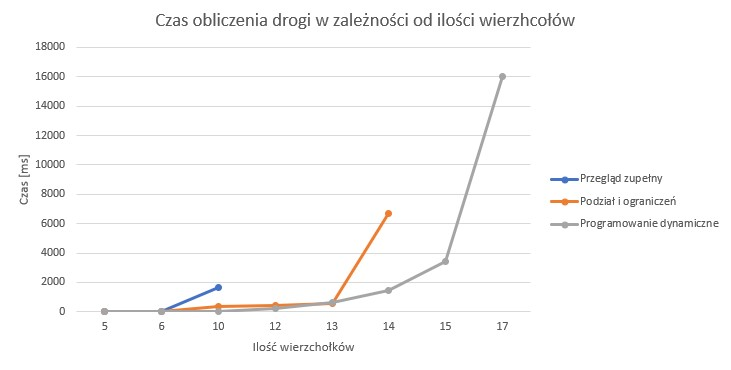
\includegraphics[width=1\textwidth]{./w.jpg}
      				\caption{Pomiary w [ms] w zależności od ilości wierzchołków}
      			\label{fig:obraz}
			\end{center}
		\end{figure}

Jak widać algorytmy przeglądu zupełnego i podziału i ograniczeń okazują się nieefektywne już przy odpowiednio 12 i 15 wierzchołkach. Ponadto algorytm podziałów i ograniczeń mimo większej wydajności zużywa dużo więcej pamięci, a jego szybkość nie jest stała - zależna od grafu jak i ilości wierzchołków grafu. Najlepsza okazała się metoda programowania dynamicznego, a przy okazji ma dużo mniejszą złożoność pamięciową 

\end{document}

